\documentclass[a4paper]{llncs}
%\usepackage{fullpage}
%\usepackage{palatino}

\usepackage{makeidx}
\usepackage{amsmath}   
\usepackage[retainorgcmds]{IEEEtrantools}
\usepackage{thumbpdf}
\usepackage{multicol}   
\usepackage{graphicx}   
\usepackage{listings}
\usepackage{algorithm}
\usepackage{algorithmic}

\usepackage[
  pagebackref,
  pdfpagelabels,
  extension=pdf,
]{hyperref}
\hypersetup{ 
  pdftitle          = {Exploring the Small-World Effect in Reinforcement Learning},
  pdfsubject        = {Exploring the Small-World Effect in Reinforcement Learning},
  pdfauthor         = {Arun Chaganty},
  pdfkeywords       = {},
  pdfcreator        = {pdflatex},
  pdfproducer       = {LaTeX with hyperref and thumbpdf},
  pdfstartpage      = {1},
  pdfpagemode       = UseThumbs,
  colorlinks        = true,
  linkcolor         = red,
  anchorcolor       = red,
  citecolor         = blue,
  filecolor         = red,
  urlcolor          = red
}

% Section References
\newcommand{\secref}[1] {\hyperref[#1]{Section~\ref*{#1}}}
\newcommand{\thmref}[1] {\hyperref[#1]{Theorem~\eqref*{#1}}}
\newcommand{\lmref}[1] {\hyperref[#1]{Lemma~\eqref*{#1}}}
\newcommand{\algoref}[1] {\hyperref[#1]{Algorithm~\ref*{#1}}}
\newcommand{\eqnref}[1] {Equation \eqref{#1}}
\renewcommand{\algorithmiccomment}[1]{\textit{// #1}}
%\theoremstyle{plain} \newtheorem{thm}{Theorem}

%Math Operators
\DeclareMathOperator {\argmax} {argmax}
%\DeclareMathOperator {\Pr} {Pr}
\DeclareMathOperator {\sgn} {sgn}
\DeclareMathOperator {\trace} {tr}
\DeclareMathOperator {\connected} {connected}
\DeclareMathOperator {\dist} {d_l}

\newcommand{\ud}{\, \mathrm{d}}
\newcommand{\diff}[1] {\frac{\partial}{\, \partial #1}}
\newcommand{\diffn}[2] {\frac{\partial^{#2}}{\, \partial {#1}^{#2}}}
\newcommand{\tuple}[1] {\langle #1 \rangle}

%Short hand
\newcommand{\mdp} {\ensuremath{\mathcal{M}}}
\newcommand{\states} {S}
\newcommand{\actions} {A}
\newcommand{\transitions} {P}
\newcommand{\rewards} {R}
\newcommand{\Rewards} {\mathcal{R}}
\newcommand{\graph} {\mathcal{G}}
\newcommand{\policy} {\pi}
\newcommand{\initset} {\mathcal{I}}
\newcommand{\stopcond} {\beta}
\newcommand{\option} {\tuple{ \initset,\policy,\stopcond} }
\newcommand{\options} {\mathcal{O}}


\title{Exploring the Small-World Effect in Reinforcement Learning}
\author{ Arun Tejasvi Chaganty \inst{1} \and Prateek Gaur \inst{1} } 
\institute{ Department of Computer Science and Engineering, \\
            IIT Madras, Chennai, India - 500084 }

\pagestyle{headings}  % switches on printing of running heads

\frontmatter
\mainmatter

\begin{document}

\maketitle
%\pagebreak

% Outline
\begin{abstract}
    Dolors Ipsum elors
\end{abstract}

\section{Introduction}
\label{sec:intro}

% RL - challenges - need for structure
Reinforcement learning (RL) is a widely studied learning framework for
autonomous agents, particularly because of it's extreme generality; it
addresses the problem of learning optimal agent behaviour in an unknown
stochastic environment. In this setting, an agent explores a state
space, receiving rewards for actions it takes; the objective of the
agent is to maximise it's rewards accumlated over time. However, when
scaling up to larger domains, these agents require prohibitively large
amounts of experience in order to learn a good policy. By allowing the
agent to exploit the structure of environment or task, we can reduce the
experience required.

% Types of structure - temporal abstractions - options
Structure can be imposed on a learning task through either spatial or
temporal abstractions. With the former, the state-space is minimised
using information about the symmetries present in the domain.
\cite{Li2006} provides a survey of such approaches. In the latter case,
high-level actions are introduced which capture sequences of primitive
actions. In this light, temporal abstractions capture the notion of
a ``subtask''. The most common approach for temporal abstractions is the
options framework proposed by Sutton, Precup and Singh
\cite{SuttonPrecupSingh1998}, and we build our work on this framework
also. Work by Ravindran on relativised options \cite{Ravindran2003} show
how temporal abstractions can be combined with spatial abstractions.
Both spatial and temporal abstractions play an important role in
transfer learning, where we wish to extend optimal behaviour learnt in
one task to another task; a survey of such techniques can be found in
\cite{Taylor2009a}.

% Getting options - related work - deficiency
While options provide a broad framework for temporal abstraction, there
is still no consensus on how to choose subtasks. The prevalent view is
that subtasks should represent skills, i.e. partially defined action
policies that constitute a part of many reinforcement learning problems
\cite{Thrun1995}. For this reason, much of the existing work centres
around identifying `bottlenecks', regions that the agent tends to visit
frequently \cite{McGovern2001}, either empirically as in
\cite{McGovern2001}, or, more recently, using graph theoretic methods
like betweenness centrality \cite{Simsek2008} or graph partitions
\cite{Menache2002}. The intuition is that options that navigate an agent
to such states helps the agent move between strongly connected
components, thus leading to efficient exploration. 

\draft{Refine}
These option generation schemes suffer two serious drawbacks; (i)
inapplicable without bottlenecks, (ii) explode the decision space, (iii)
require complete information of the MDP.

If one considered these options as additional edges to the bottleneck
states, the resultant state-interaction graph would now be ``more''
connected. To highlight the importance of the connectivity of the
state-interaction graph, consider the Markov chain induced by a policy
for an Markov decision process. It is well known that the convergence
rate of a Markov chain (mixing time), is directly related to its
conductance \cite{Jerrum1988}, and thus its algebraic connectivity.

% Motivation for small world
Recognising the importance of connectivity, we try to apply concepts
from Kleinberg's work on small world networks, which have been shown to
have exceptionally high algebraic connectivity, and thus fast Markov
chain mixing times \cite{Salehi2007}, to the context of problem solving
with autonomous agents. Small-world networks have found diverse
applications from sensor networks, to load balancing, to swarms
\cite{Saber2005}. A small-world network has the property that an agent
can discover a short path to any destination using only local
information \cite{Kleinberg2000}; by contrast, other graph models with
a small diameter only state the existence of a short path, and do not
guarantee that an agent would be able to find such a path.  

In our context, we construct subtasks distributed according to the small
world distribution as follows; create an option that will take the agent
from a state $s$ to another state $s'$ with a probability inversely
proportional to the distance between $s$ and $s'$.We are able to prove
that this set of subtasks enables the agent to easily solve any task by
using only a logarithmic number of options to reach a state of maximal
value (\secref{sec:theory}). As this scheme adds at most one additional
option per state, we do not explode the decision space for the agent.

Furthermore, in \secref{sec:algo}, we devise an algorithm that learns
options according to the small world distribution from the optimal
policies learnt on only a couple of tasks in the domain. Thus not only
are small world options effective to use, they are also simple to learn,
and do not require any knowledge of the MDP, nor do they need to
construct a model. 

Experiments on several standard domains show that small-world options
outperform bottleneck-based methods, even when using suboptimal option
policies. \draft{Do the contributions need to be made explicit?}

\draft{Is this required?} The remainder of the paper is organised as follows. We present an overview of reinforcement learning, and the options framework in \secref{sec:background}. We then define a small world option, and prove that given such options, an agent will require to use only a logarithmic number of them to perform a task in \secref{sec:theory}. From a more practical perspective, we present an algorithm to extract these options from optimal policies learnt on several tasks in the domain in \secref{sec:algo}. We present our experimental results in \secref{sec:experiments}. Finally, we conclude in \secref{sec:conclusions}, where we present future directions for our work. \appendixref{sec:small-world-theory} contains an extension of Kleinberg's proof for the distributed search property of small-world networks which is used in \secref{sec:theory}.


\section{Motivation}
\label{sec:motivation}

% Cognitive perspective 
% Social Networks Perspective - distributed search


\input{algorithm}
\section{Experimental Results}
\label{sec:experiments}
% Experimental results

We trained MacroQ learning agents on several standard domains, and
measured the cumulative return obtained using the following option
generation schemes: 
\begin{itemize}
   \item \textbf{None}: No options were used.
   \item \textbf{Random}: Options were generated by randomly connecting
     two nodes in the domain (this is equivalent to $P_0$.
   \item \textbf{Betweenness}: As a representative of bottleneck-based
     schemes, options were generated to take any node to a local maxima
     of betweenness centrality, as described in \cite{Simsek2008}. 
   \item \textbf{Small World}: Options were generated randomly
     connecting two nodes of the domain using an inverse square law, as
     described in \secref{sec:theory}.
\end{itemize}

Each experiment, unless mentioned otherwise, was run for $10$ randomly
generated tasks in the domain; each task ran for $40,000$ epochs, and
was averaged over an ensemble of $20$ agents.

\subsection{Optimal Options}
The agents were run on the following three domains using the algorithm
sketched in \secref{sec:theory}:
\begin{itemize}
   \item \textbf{Arbitrary Navigation}: The agent must reach an
     arbitrary goal state in an obstacle-free $x \times y$ grid-world. 
   \item \textbf{Rooms}: The agent must navigate a floor plan with
     4 rooms to reach an arbitrary goal state.
   \item \textbf{Taxi}: This is the domain described in
     \exref{example:taxi}.
\end{itemize}

The results of these experiments are summarised in
\autoref{tbl:optimal-returns}. Small world options perform significantly
better than the other schemes in navigation-oriented tasks like Rooms or
Arbitrary Navigation. In the Taxi domain, options generated by the
betweenness scheme outperform the small world options. This is expected
because the goal states in this domain lie at betweenness maxima.

\begin{figure*}[th]
    \center
    \subfigure[Options Learnt]{
      \includegraphics[height=2in]{figures/rooms-options}
      \label{fig:rooms-options}
    }
    \subfigure[Cumulative Return (with 200 options)]{
      \includegraphics[height=2in]{figures/rooms-return-200}
      \label{fig:rooms-return}
    }
    \caption{The Rooms Domain}
\end{figure*}

Some of the small world options preferred in Rooms domain are shown in
\figref{fig:rooms-options}. The graph shows several examples of options
that compose together to arrive near the goal state. We have also
plotted the learning behaviour in \figref{fig:rooms-return}. 

\begin{figure*}[th]
    \center
    \subfigure[$k$ vs Cumulative Return]{
      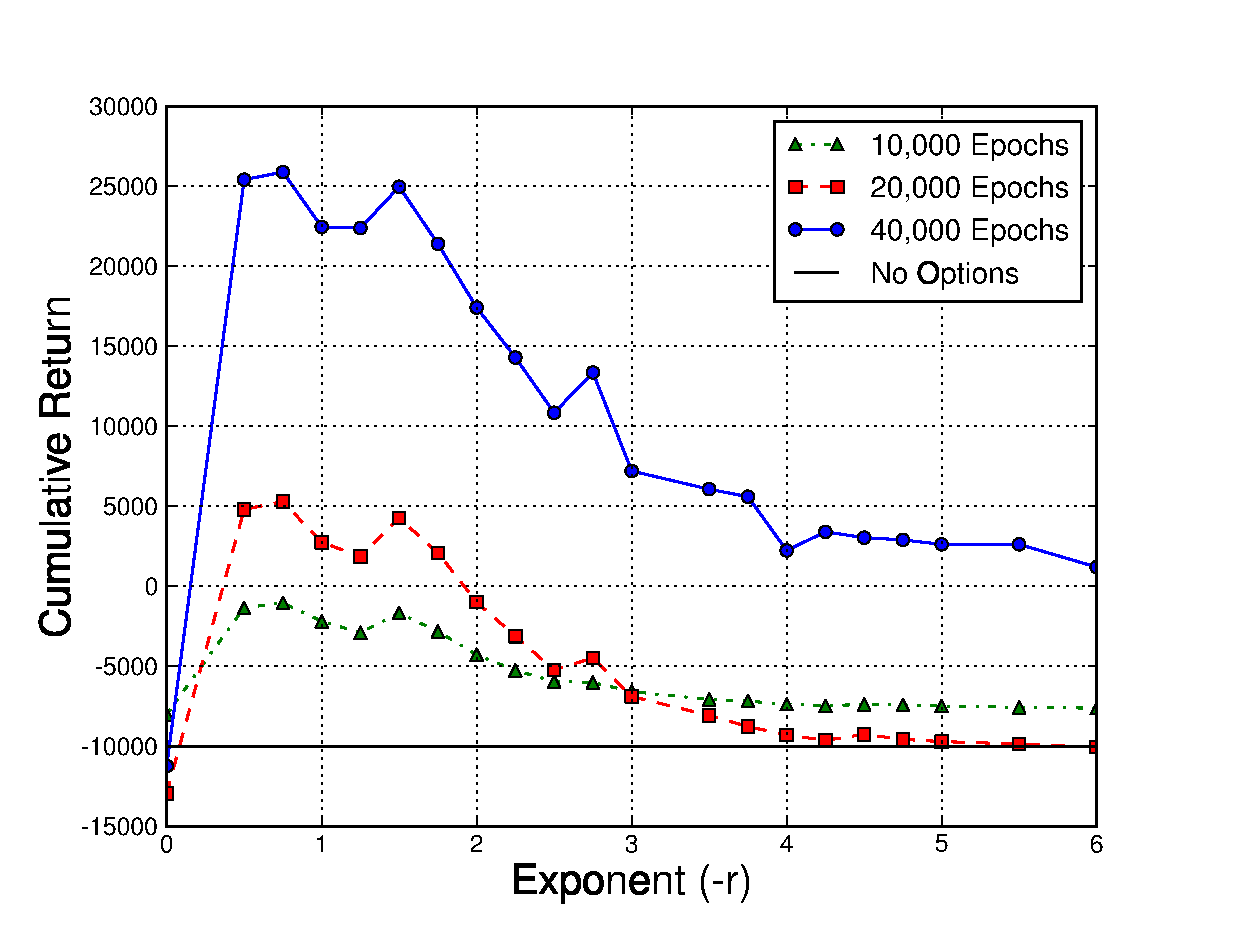
\includegraphics[height=2in]{figures/rooms-exp}
      \label{fig:rooms-exp}
    }
    \subfigure[Options Learnt on a Budget]{
    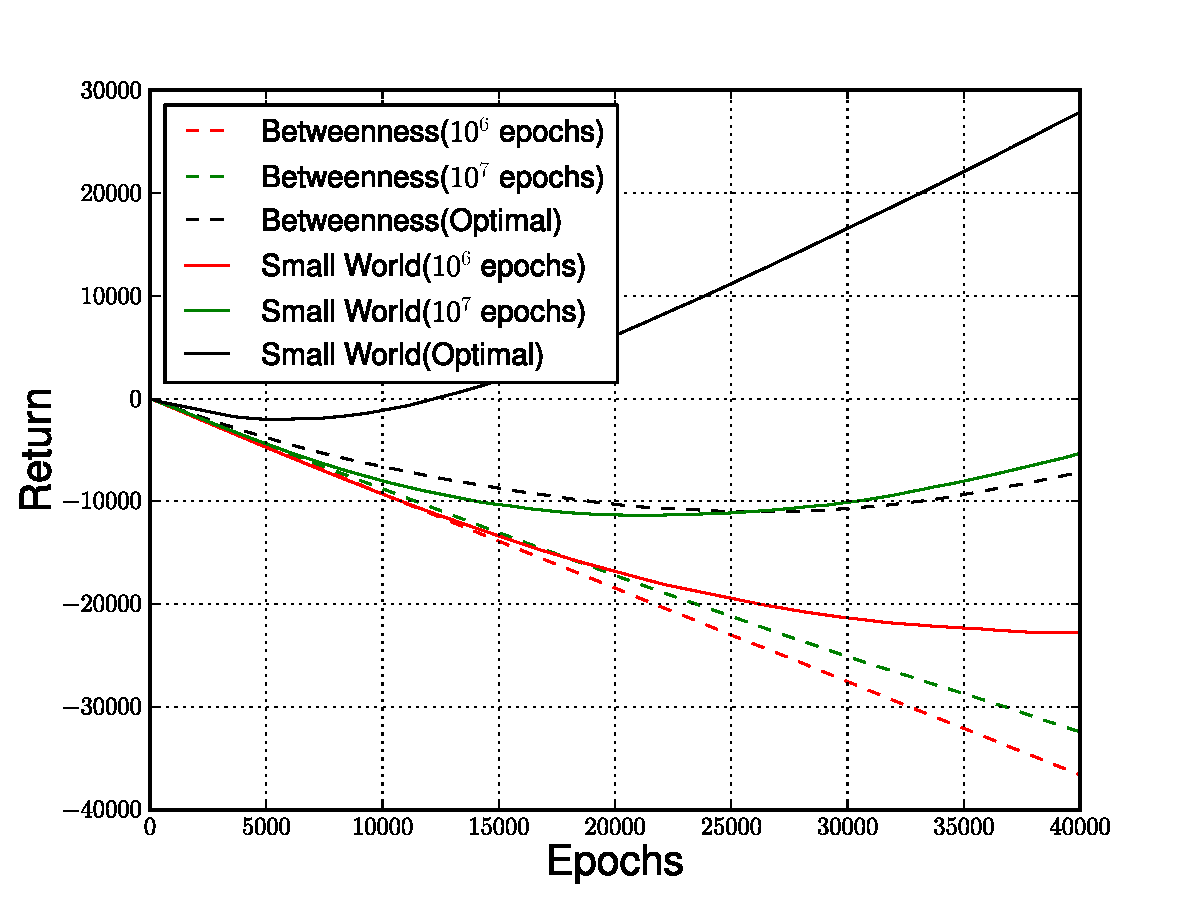
\includegraphics[height=2in]{figures/rooms-learnt-200}
      \label{fig:rooms-learnt}
    }
    \caption{The Rooms Domain (contd.)}
\end{figure*}

\subsection{Effect of $k$}
We do not yet have a clear understanding of how the exponent $k$ should
be chosen. \figref{fig:rooms-exp} plots $k$ versus the cumulative return
on the Rooms domain. The performance of the agent without options after
$20,000$ epochs is also plotted for reference. There is a range of $k$
($\approx 0.75$ to $1.5$) with good performance, after which the
performance steadily drops. This behaviour is easily explained; as the
exponent goes up, the small world options generated are very short, and
do not help the agent get nearer to the maximal value state. The optimal
range of $k$ is slightly counter-intuitive because the Rooms domain is
a two dimensional lattice with some edges removed. As a consequence of
the reduced connectivity, and perhaps due to stochastic factors, longer
range options are preferred.

\subsection{Options Learnt on a Budget}
In \secref{sec:algo}, we describe an algorithm to construct small world
options efficiently when given a limited number of learning epochs. We
compared the performance of these options with betweenness options
learnt similarly, and have plotted our results in
\figref{fig:rooms-learnt}. Despite using many more
options, the small world options thus created significantly outperform
betweenness options learnt with the same budget, and are even comparable
to the optimal betweenness options.


\section{Conclusions and Future Work}
\label{sec:conclusions}

% Contributions
% - new scheme for generating options
We have devised a new scheme to generate options based on small world
network model. The options generated satisfy an intuitive criteria, that
the subtasks learnt should be easily composed to solve any other task.
The options also greatly improve the connectivity properties of the
domain.

% - absolutely model-free
Experiments run on standard domains show significantly faster learning
rates using small world options. At the same time, we have shown that
learning small world options can be significantly cheaper than learning
`bottleneck' options. Another advantage of the scheme is that is does
not ever require the model of the MDP. We find it remarkable that we can
learn near optimal behaviour just from the policies of on some tasks


% - theoretical interest
The scheme does not perform any global analysis, and does not require
the model. We have shown that sample-wise, it can be far cheaper than
other bottleneck based methods. Does not lead to state space blow up.
Also is interesting from a theoretical perspective, logarithmic number
of decisions.

% Further work
% - dynamically add/remove options
% - figuring out r
We have as yet not been able to characterise what the exponent $r$
should be in a general domain. Given the ease with which options can be
discovered, it would be interesting to create a dynamic scheme.



\bibliography{library}{}
\bibliographystyle{alpha}

%\newpage
%\appendix

%
\section{Code}
\label{sec:code}
% \lstset{language=TCL, basicstyle=\small, showstringspaces=false, numbers=left, numberstyle=\tiny }
% \lstinputlisting{many2one.tcl}


\end{document}

